

De gate van de MOS transistor is ge\"isoleerd van het geleidende kanaal door middel van het gate oxide, die een capaciteit heeft van:
\begin{equation}
C\tss{ox} = \frac{\epsilon\tss{ox}}{t\tss{ox}}
\end{equation} 
waarbij \emph{$\epsilon$\tss{ox}} de permittiviteit is van het oxide en \emph{t\tss{ox}} de dikte is van het oxide.
\\
De totale waarde van deze capaciteit heet de gate capaciteit \emph{C\tss{G}} en hangt onder andere af van de overlap capaciteit per lengte-eenheid \emph{C\tss{o}} en de gate-channel capaciteit per oppervlakte-eenheid \emph{C\tss{GC}}. Ook spelen de breedte \emph{W} en de lengte \emph{L} een rol. De volgende formule geeft het verband weer tussen deze variabelen:
\begin{equation}
C\tss{G} = W \ast C\tss{o} + L \ast W \ast C\tss{GC}
\end{equation}
De overlap capaciteit is de capaciteit die ontstaat doordat de grenzen van de source en de drain een klein stukje onder de gate zitten. Aangezien de gate en de source en drain van lading verschillen ontstaat hier een capaciteit die afhangt van de breedte \emph{W}. De \emph{G\tss{GC}} hangt af van de \emph{$\epsilon$\tss{ox}} en de t\tss{ox}, dus:
\begin{equation}
C\tss{GC} = C\tss{ox} = \frac{\epsilon\tss{ox}}{t\tss{ox}}
\end{equation}
Stel nu dat wij een schakeling maken zoals in figuur \ref{res:RABAEY_SCHAKELING} en het resultaat plotten in een grafiek met op de y-as de gate capaciteit \emph{C\tss{GC}} en op de x-as gate source spanning \emph{V\tss{GS}}. Dan ziet de grafiek eruit als in figuur \ref{res:RABAEY_CAP_PLOT}.

 \begin{figure} [h!]
 \begin{center}
 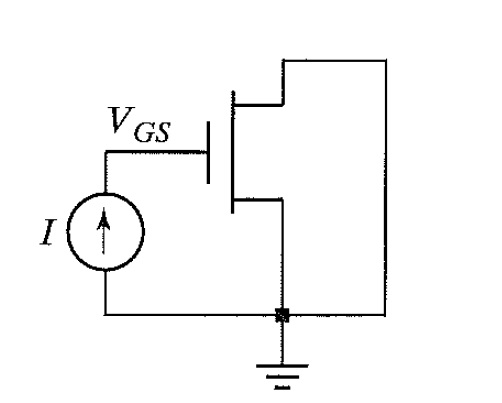
\includegraphics [scale = 0.7] {figures/RABAEY_SCHAKELING}
 \caption{Circuit om de gate capaciteit te bepalen van een NMOS transistor in 25$\mu$m technologie uit Rabaey [1]}
 \label{res:RABAEY_SCHAKELING}
 \end{center}
 \end{figure}

 \begin{figure} [h!]
 \begin{center}
 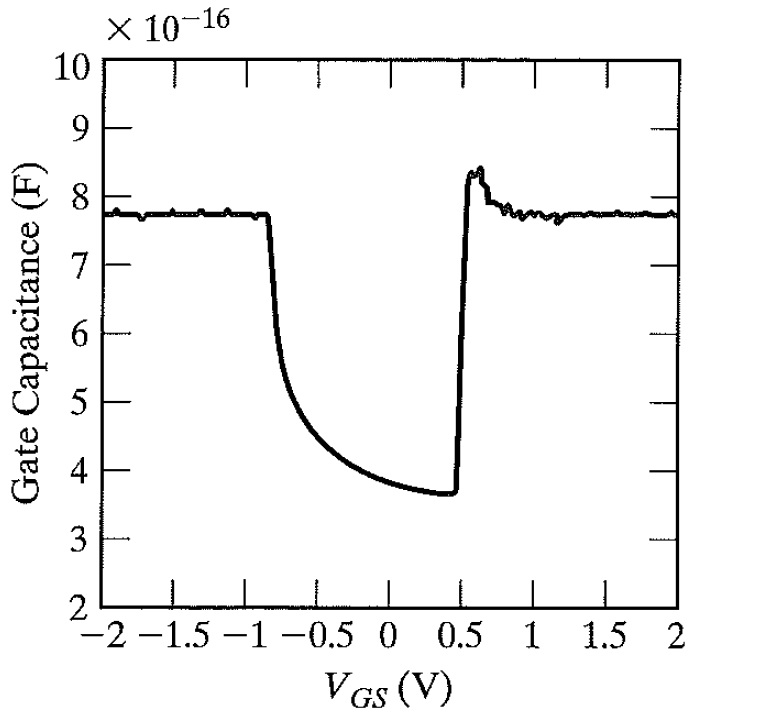
\includegraphics [scale = 0.4] {figures/RABAEY_CAP_PLOT}
 \caption{Plot van de \emph{C\tss{GC}}  \emph{V\tss{GS}} van een NMOS transistor in 25$\mu$m technologie uit Rabaey [1]}
 \label{res:RABAEY_CAP_PLOT}
 \end{center}
 \end{figure}

Uit figuur \ref{res:RABAEY_CAP_PLOT} is duidelijk te zien dat de \emph{C\tss{GC}} niet constant is voor elke \emph{V\tss{GS}}. Dit komt door de verschillende werkgebieden van de transistor. In figuur \ref{res:RABAEY_REGIONS} is een schematische weergave gegeven van drie verschillende werkgebieden. De verandering in capaciteitswaarde van de \emph{C\tss{GC}} is als volgt te verklaren: in het eerste vlakke gedeelte van figuur \ref{res:RABAEY_CAP_PLOT} zit de weerstand in het cut-off werkgebied. Er loopt geen stroom tussen source en drain. Naarmate de \emph{V\tss{GS}} stijgt, wordt de \emph{C\tss{GC}} kleiner. Dit komt omdat het p-substraat dat onder het gate oxide zit steeds verder naar beneden wordt gedrukt. Hierdoor wordt de afstand groter en dus de \emph{C\tss{GC}} kleiner. Zodra de \emph{V\tss{GS}} verder stijgt komt de transistor in het resistieve gebied. In dit gebied gaat een stroom tussen source en drain lopen. Hierdoor bereikt de \emph{C\tss{GC}} een constante waarde. Uit deze constante waarde kan men de dikte van het oxide afleiden. Het saturatie werkgebied van de transistor is voor dit verslag niet van belang en zal daarom hier niet worden besproken.

 \begin{figure} [h!]
 \begin{center}
 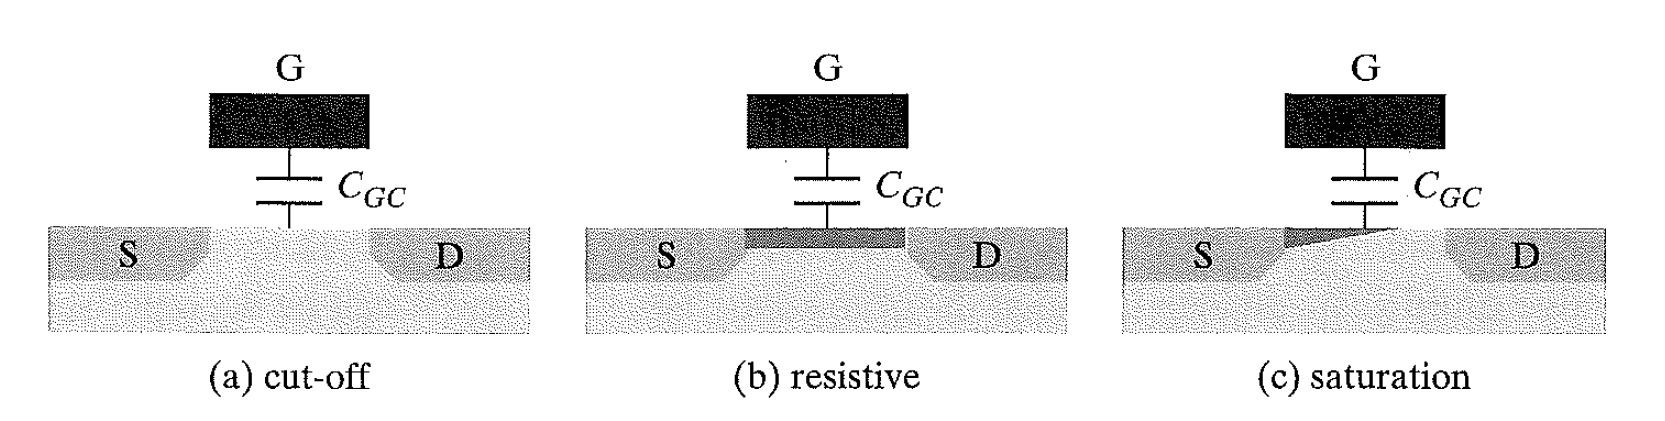
\includegraphics [scale = 0.4] {figures/RABAEY_REGIONS}
 \caption{Drie verschillende werkgebieden van een NMOS transistor uit Rabaey [1]}
 \label{res:RABAEY_REGIONS}
 \end{center}
 \end{figure}





























